\documentclass[10pt]{beamer}

\usepackage{amsmath}
\usepackage{graphicx}
\usepackage{subfig}

\setbeamertemplate{caption}[numbered]


\author{Marco}
\title{Beamer Example}
\institute{UZH}
\date{today is \MakeLowercase{\today}}

\begin{document}
	\begin{frame}
		\titlepage
	\end{frame}
%--------------------------------------------------
	\begin{frame}
		\frametitle{Content}
		\tableofcontents
	\end{frame}
%--------------------------------------------
\begin{frame}
\section{Introduction}
\frametitle{Slide with Equations}
\framesubtitle{Using package amsmath}
	\begin{gather}
	  	e^{\pi i}  - 1 = 0 \\
	 	 g = 10 m/s^2
	\end{gather}



\end{frame}
%----------------------------------------------------
\begin{frame}
\section{Slide with Proof}
\frametitle{Slide with Proof}
\framesubtitle{Using the Theorem Environment}

	\begin{theorem}
	Let \(f\) be a function whose derivative exists in every point, then \(f\) 
	is a continuous function.
	\end{theorem}
	See figure \ref{figure1}:

	\begin{figure}
		\centering 
		\subfloat[\centering Bad Function]{{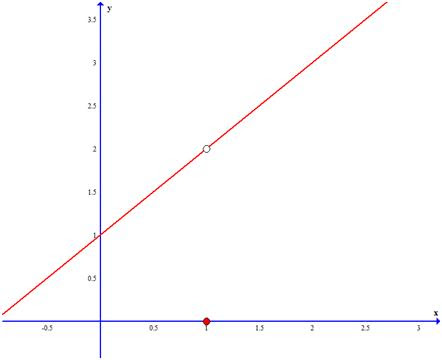
\includegraphics[width = 3cm]{figure.jpg} }}
		\qquad
		\subfloat[\centering Good Function]{{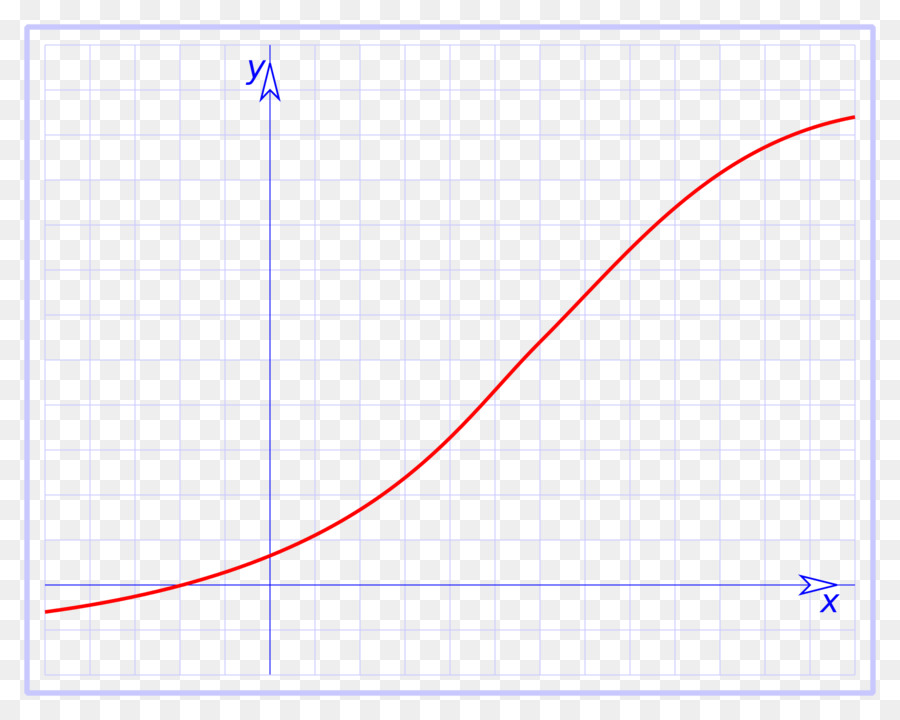
\includegraphics[width = 3cm]{figure2.jpg} }}
		\caption{Good and Bad functions}
		\label{figure1}
	\end{figure}

\end{frame}

%-----------------------------------------------------
\begin{frame}
\section{Conclusion}
\frametitle{conclusion}
\end{frame}

\end{document}
